\documentclass[tikz,border=7pt]{standalone}
\usetikzlibrary{calc}
\begin{document}
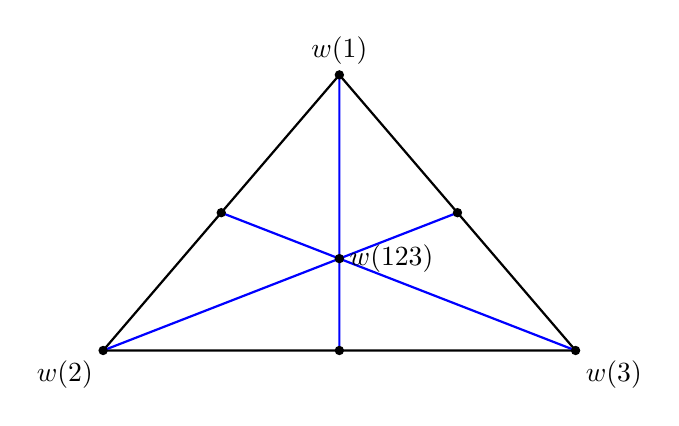
\begin{tikzpicture}[line width=.8pt]
\coordinate (A) at (0,3.5); \coordinate (B) at (-3,0); \coordinate (C) at (3,0);
\coordinate (AB) at ($(A)!.5!(B)$); \coordinate (BC) at ($(B)!.5!(C)$); \coordinate (CA) at ($(C)!.5!(A)$);
\coordinate (G) at (0,1.1667);
\draw (A)--(B)--(C)--cycle; \draw[blue,thick] (A)--(BC) (B)--(CA) (C)--(AB);
\foreach \p in {A,B,C,AB,BC,CA,G} \fill (\p) circle (1.7pt);
\node[above] at (A) {$w(1)$}; \node[below left] at (B) {$w(2)$}; \node[below right] at (C) {$w(3)$};
\node[right] at (G) {$w(123)$};
\end{tikzpicture}
\end{document}
